\documentclass[12pt,letterpaper,twoside]{amsart}
\usepackage[latin1]{inputenc}
\usepackage{amsmath}
\usepackage{amsfonts}
\usepackage{graphicx}
\usepackage{amssymb}
\usepackage{multicol}
\usepackage{ulem}
\newcounter{example}
\newcounter{exercise}
\newcounter{problem}
\newtheorem{theorem}{Theorem}
\newcommand{\example}{\bigskip \noindent {\large {\sc Example \arabic{example}:}} \addtocounter{example}{1}}
\newcommand{\exercise}{\bigskip \noindent {\large {\sc Exercise \arabic{exercise}:}} \addtocounter{exercise}{1}}
\newcommand{\problem}{\bigskip \noindent {\large {\sc Problem \arabic{problem}:}} \addtocounter{problem}{1}}
\newcommand{\tech}{\marginpar{\vskip 10mm \begin{center}\includegraphics[width=0.25in]{calculatorimagesmall.eps} \end{center}}}
\newcommand{\solution}{\medskip \noindent {\bf Solution: }}
\newcommand{\R}{\mathbb{R}}





\begin{document}

\sffamily

%%%%  switch the commenting on this line and the next \chapter{Introduction}
\begin{center} {\LARGE Graphical Methods} \end{center}

\setcounter{example}{1}
\setcounter{exercise}{1}

In this chapter, we introduce some methods for obtaining a qualitative understanding of solutions to differential equations.  These methods are especially useful when it is difficult or impossible to calculate an explicit formula for a solution.

The first tool we will discuss is a {\bf direction field}, also called a {\bf slope field} for an ODE.  An ODE in the form $\frac{dy}{dx}=f(x,y)$ defines a slope at each point of the xy-plane.  We can graph small line segments (or vectors) at a lattice of points in the plane in order to illustrate how a solution should behave if it goes through that point.

\example Consider the ODE $y'=3y+x$.  The following plot is a slope field for this differential equation.

\begin{center}
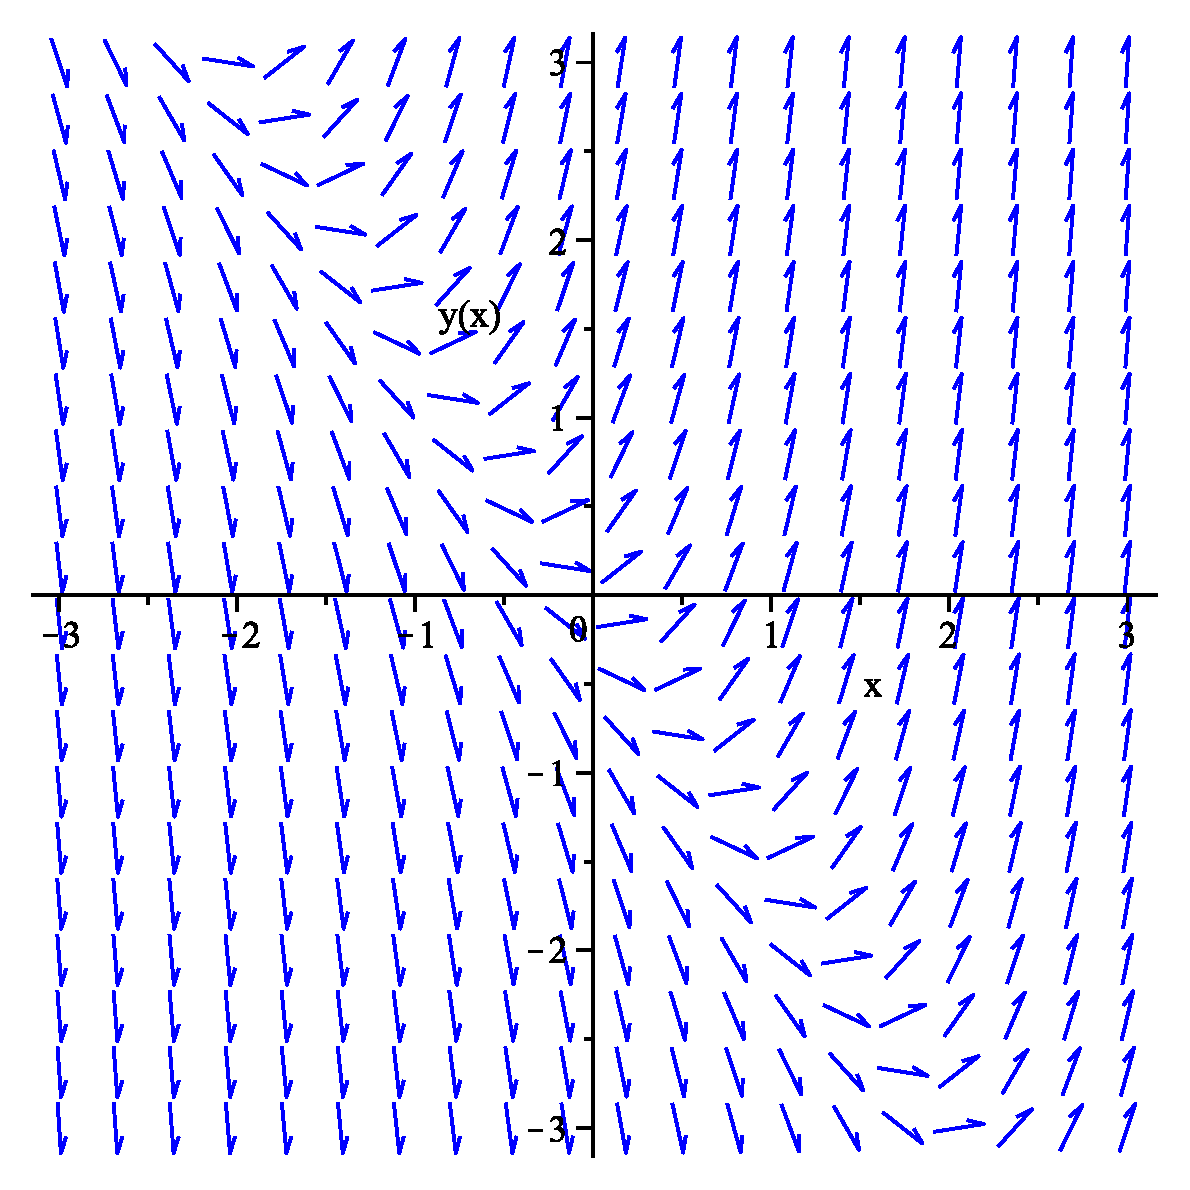
\includegraphics[width=3in]{slopefield1.eps}
\end{center}

The vectors indicate the tangent lines to graphs of solutions curves.  For example, if a solution $y(x)$ of this ODE has a graph that passes through the point $(0,1)$, then the slope of that curve will be $1$ at that point, because $y'=3(1)+(0)=3$, according to the differential equation $y'=3y+x$.  We will be able to verify this fact analytically once we know how to write down an explicit solution for this initial value problem: $y=-\frac{1}{9}-\frac{x}{3}+\frac{10}{9}e^{3x}$.  Indeed, we see that $y'=-\frac{1}{9}+\frac{10}{3}e^{3x}$, and at $x=0$ we get $y'=3$.  The following plot shows the graph of this solution $y(x)$ superimposed on the slope field.

\begin{center}
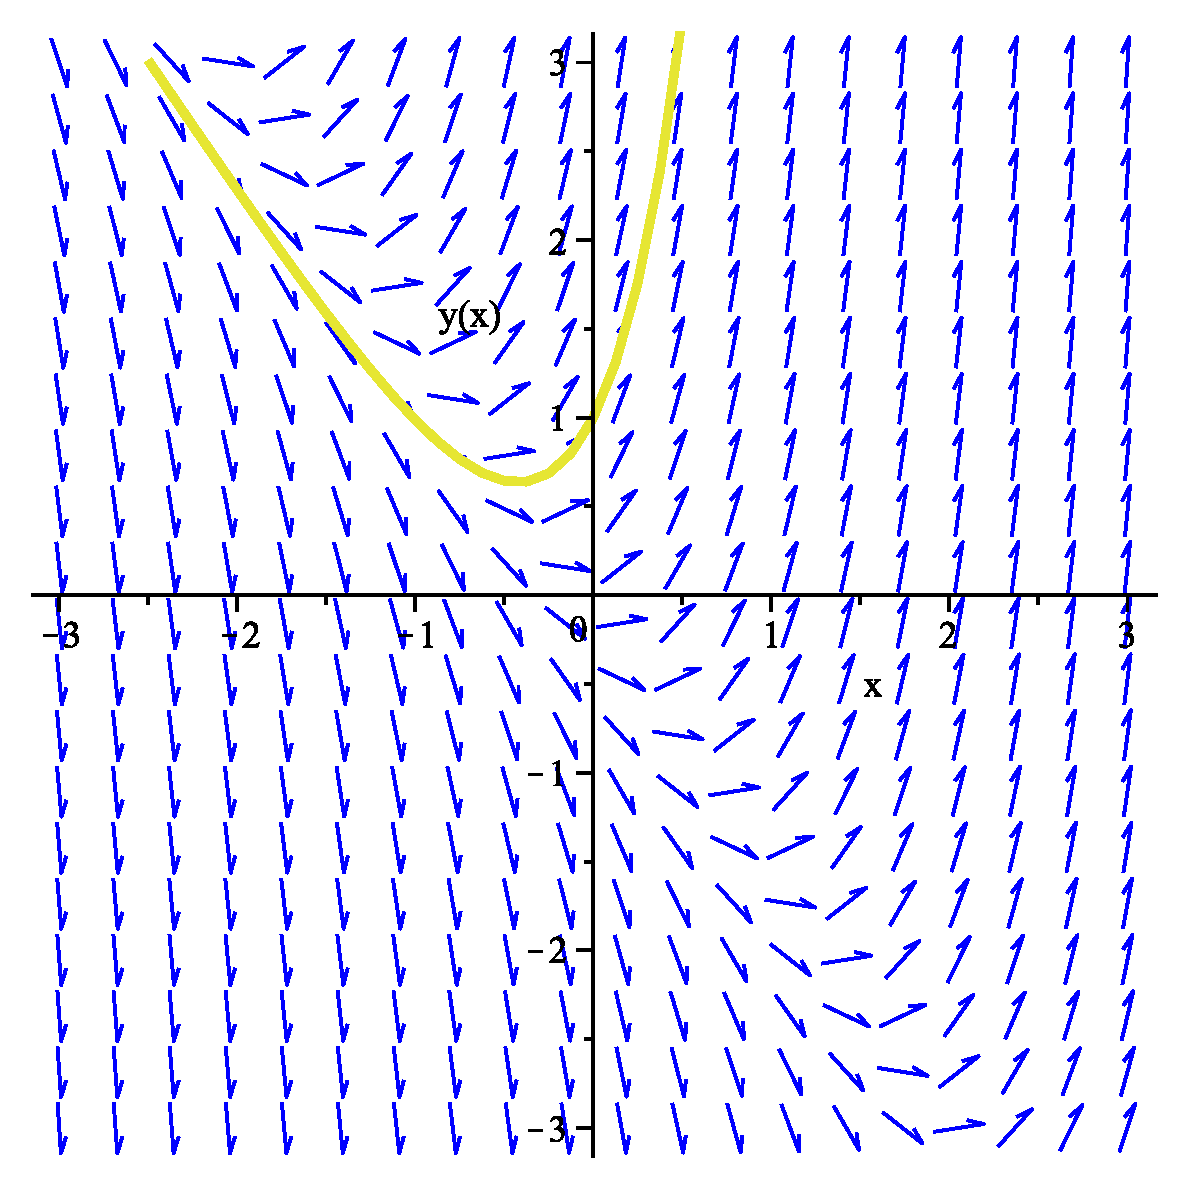
\includegraphics[width=3in]{slopefield2.eps} 
\end{center}

With a slope field, we can explore the behaviour of solutions {\it without} having an explicit formula for the solution.  For example, we could see from the slope field above that if a solution passed through the point $(0,1)$, then as $x$ increases so will $y$.  We can even guess that $\lim_{x \rightarrow \infty} y(x)=\infty$ (provided that the interval of definition of $y$ extends all the way to infinity).

In contrast, imagine a solution of $y'=3y+x, \ y(0)=-1$ is graphed on top of the slope field.  Then the solution will be decreasing at first as x increases. The plot below shows a curve that passes through $(0,-1)$ and whose tangent lines at each point are parallel to the slope field at each point.  This graph is our sketch of a solution to the initial value problem.

\begin{center}
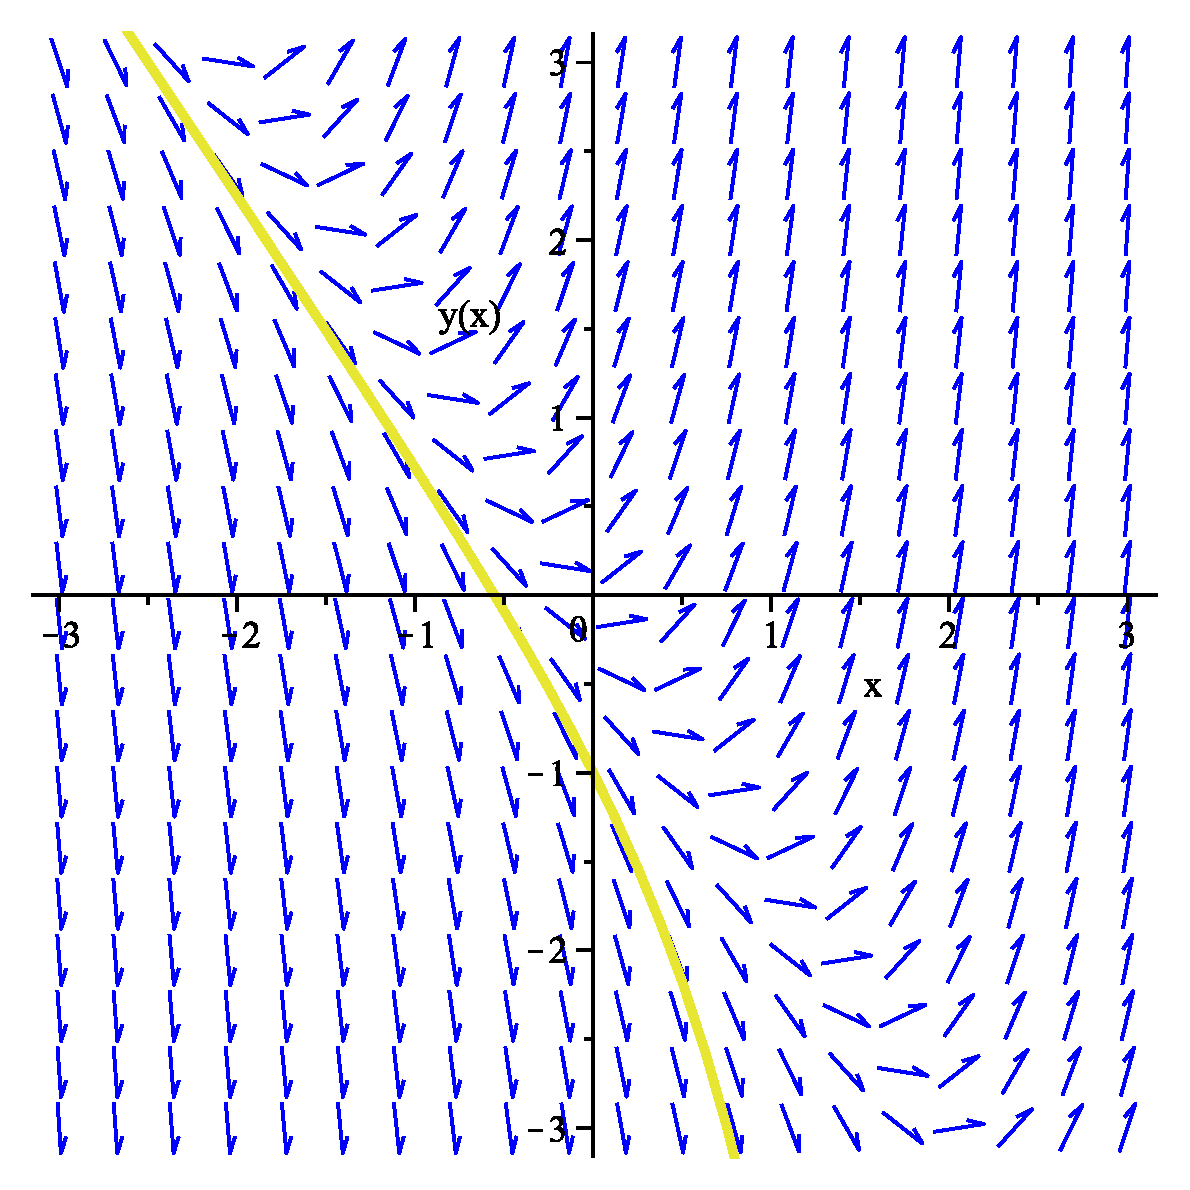
\includegraphics[width=3in]{slopefield3.eps}
\end{center}

Slope fields can be generated by hand, but it is usually much more efficient to use a computer program to generate them.  

\exercise Generate a slope field for $y'=y(y-2)$.  Then sketch several solution curves on the plot: one for each of the following initial conditions: $y(0)=-1$, $y(0)=0$, $y(0)=1$, and $y(0)=2$.  In each case, use the behaviour you see on the slope field to predict the value of $\lim_{x \rightarrow \infty} y(x)$. 

\exercise Use a slope field to predict the behaviour of $\lim_{x \rightarrow \infty} y(x)$, where $y$ is a solution of $y'=y+4$.  Explain how this limit depend on the initial value $y(0)$.

\exercise Use a slope field to predict the behaviour of $\lim_{x \rightarrow \infty} y(t)$ where $y$ is a solution of $\dot{y}=y-t$, $y(0)=0$

\exercise Use a slope field to predict the behaviour of solutions to $y'=y^2$.  Then confirm your prediction by finding a formula for the solution of the initial value problem $y'=y^2, \ y(0)=y_0$.  {\it (Hint: Use separation of variables.)}

\bigskip
Slope fields also provide us with some intuition regarding the existence and uniqueness of solutions.  It seems like, given a slope field representing a differential equation of the form $\frac{dy}{dx}=f(x,y)$ and a point in the plane $(x_0,y_0)$ representing the initial condition, we ought to be able to find a curve through that point that follows the slope field.  This suggests that initial value problems of the form $y'=f(x,y), \ y(x_0)=y_0$ ought to have solutions (at least in some interval containing $x_0$).  Indeed, if $f(x,y)$ is a nice function, then this is the case, and we will give a rigorous proof of this fact in a later chapter.  

Notice that the easiest slope fields to plot, if we need to do so by hand, are the ones where the right side of the differential equation depends on only one variable, such as $\frac{dy}{dx}=f(y)$, because all the direction vectors along a horizontal line have the same slope.  These have a special name: we say that a differential equation of the form $y'=f(y)$ is {\bf autonomous}.

Incidentally, equations of the form $y'=g(x)$ also have slope fields that are easy to plot, since the direction vectors along any vertical line have the same slope; however, these equations are not of as much interest to us in this course since they were studied extensively in calculus -- a solution of $y'=g(x)$ is just an antiderivative of the function $g$.

Next, we turn our attention to another graphical approach for understanding solutions of differential equations that is specifically applicable to autonomous equations.

\example Suppose the velocity $v(t)$ (in meters per second) of a falling object that encounters air resistance is modelled by the differential equation
\[ \dot{v} = 9.8-Kv\]
where $K>0$ is a constant.  The idea here is that air resistance is a force that is proportional to the speed of the object, and so the constant of proportionality K here depends on both the speed and the mass of the falling object; the $9.8$ account for the acceleration due to gravity, and by selecting a positive quantity here, we have implicity assume that positive velocities correspond to {\it downward} motion.  

Let us graph $\dot{v}$ as a function of $v$:

\begin{center}
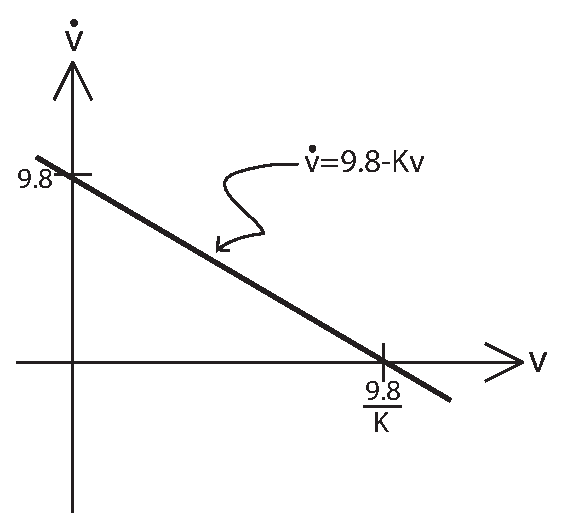
\includegraphics[width=4in]{phaseline1.eps}
\end{center}

The graph intersects the $v$-axis at $v=\frac{9.8}{K}$.  According to this graph, whenever the velocity is less than $\frac{9.8}{K}$, $\dot{v}$ will be positive, and therefore the object will continue to increase its velocity.  Similarly, if the velocity were to start out above $\frac{9.8}{K}$, then $\dot{v}$ will be negative, and therefore the velocity will decrease.  In both cases, the velocity will head toward the value $v=\frac{9.8}{K} \frac{m}{s}$.  And if the initial velocity is exactly $\frac{9.8}{K} \ \frac{m}{s}$, then $\dot{v}=0$ so the velocity will remain constant. We use arrows on a number line to illustrate the behaviour of the solution as follows:

\begin{center}
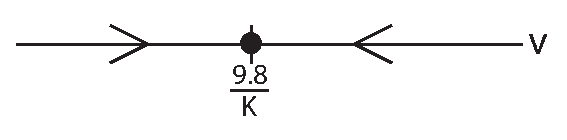
\includegraphics[width=4in]{phaseline2.eps}
\end{center}

This figure is called the {\bf phase line} for the differential equation: it indicates the constant solutions of the equation with dots (in this case, $v=\frac{9.8}{K}$ is the only constant solution), and it uses arrow to indicate the {\bf long-term behaviour} of solutions with other initial conditions.

In this application, the constant solution is called the {\bf terminal velocity} of the falling object -- it is the limiting value of the velocity as $t$ increases:
\[ \lim_{t \rightarrow \infty} v(t) = \frac{9.8}{K} \ \frac{m}{s}.\]
\qed

\exercise Suppose that an object is known from observations to have a terminal velocity of $196 \frac{m}{s}$.  Write down an initial-value problem for the velocity of this object if the initial velocity is $0 \frac{m}{s}$.

\exercise A tank contains a changing mixture of pure water and brine (salt water solution).  The differential equation that models the quantity of salt in the tank after $t$ minutes have passed is
\[ \dot{S} = 8-\frac{4S}{25} \ \frac{grams}{min}\]
where $S(t)$ is measured in grams.  Use a phase line analysis to determine the long-term behaviour, $\lim_{t \rightarrow \infty} S(t)$.




%% Cut below here for the book form.

\begin{center} {\LARGE Problems} \end{center}

\setcounter{problem}{1}

\problem Use a phase line analysis to determine the long-term behaviour of solutions to the differential equation 
\[ \dot{y} = \sin(y).\]
How does the behaviour depend on the initial value $y(0)$?

\problem Perform a phase line analysis for the logistic differential equation, $\dot{P}=kP(M-P)$.

\problem Find a differential equation $\dot{y}=f(y)$ which is consistent with the phase line shown below (there is more than one correct answer):

\begin{center}
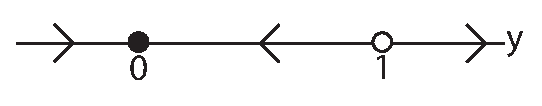
\includegraphics[width=4in]{phaseline3.eps}
\end{center} 






\end{document}